\section{Theory}
\subsection{Diffraction}
\paragraph{Principle of Huygens-Fresnel}
We will develop the theory of diffraction \cite{landau2} which will be usefull in the further progress
the theory. When start from geometrical optics, we notice that we use the approximation for the 
wavelength to be infinitely small. Taking into account the finite value of wavelength, we arrive at the
main concept of diffraction phenomena. Let's assume for an instance that the path of the light is limited by
opaque objects like an opening smaller than the beam of the light - then geometrical optics would predict 
total seperation between shadow and light after the opening. But with finite wavelengths, this seperation
is nullified by a complicated geometric intensity distribution fringing the areas of light,
depending on the shape and size of the opening. Clearly the smaller the openings are compared to the
wavelength this effects become stronger and stronger.
\begin{figure}[htpb]
    \centering
    \includegraphics[width=0.5\linewidth]{figures/beam}
    \caption{Sketch for the calculation of the intensity distribution Later. the Point $P$ denotes a distant
        point where we want to popagate the wave to, while $df$ at the surface of the aperture. For now 
        we assume the light incoming from the left side is parallel and monochromatic.}
    \label{fig:beam}
\end{figure}
\paragraph{Fraunhofer Diffraction}
We will not look at the non-dynamic case, leaving out all the factors $e^{-i\omega t}$ which can be appended
easily after if necessary. We start with a general wave incenting from the left side, with value $g(f)$ at the
surface of the aperture at a point $f$ (see figure \ref{fig:beam}). Then the wave at point $P$ due to the
outcoming wave of $f$ will
be proportional to $g(f)$, having lost
energy due to the enlarged surface proportional to $R$ and gaining a phase as well $e^{ikR}$ as well; 
the total wave at $P$ (which we denote with $\psi$) is thus the integral over the surface along d$f$: 
\begin{equation}
    \label{eq:int1}
    \psi_P \propto \int \frac{g(f) e^{ikR(f)}}{R(f)}\del f.
\end{equation}
The approximation is which can be sucessfull applied is fairly simply: For $P$ far enough away, the distance
$R$ is nearly the same for all points on the surface $f$, such that $R$ is not dependent on $f$ anymore and
we can pull it out of the integral
\begin{equation}
    \label{eq:int1}
    \psi_P \propto \int u(f) e^{ikR}\del f.
\end{equation}
The deeper point of this fairly easy assumption is that for distance $R \Rightarrow \infty$ the wavefunction
of an whatever shaped aperture is proportional to the Fourier Transform of the aperture. Lets assume
now a aperture function $g(x)$ of an one dimensional opening, then this translates into
\begin{equation}
    \psi_P \propto \mathcal{F} \left[g(k)\right ]_P
\end{equation}
where the dependency of $P$ in $g(x)$ comes from the factor $R$.
We have to think about fourier transformations before we can continue our studies.
\paragraph{Fourier Transformations}
We used the notation  $\mathcal{F} \left[g(k)\right ]_P$ which will be introduced here:
\begin{align}
f(x) &= \int_{-\infty}^{\infty} F(k)\exp(i kx)\del k\\
F(k) &= \mathcal{F}_x\left [f(x)\right ](k) =
\int_{-\infty}^{\infty} f(k)\exp(-i kx) \del x
\end{align}
The most important properties are:
\begin{align}
    \label{eq:fourier}
&\mathcal{F}\left [a f(x) + b g(x)\right ]
    = a F(k) + b G(k) 
    &\mbox{ (Linearity) }\\
&\mathcal{F}\left [f(x) * g(x)\right ](k)
    = \mathcal{F}\left [f(x)\right ]\mathcal{F}\left [g(x)\right ]
    \! &\mbox{ (Convolution) }\\
&\mathcal{F}_k\left [\left | F(k) \right |^2\right ](x)
   =  \int_{-\infty}^{\infty}\bar{f}(\tau)f(\tau + x) \del\tau 
   &\mbox{ (Wiener-Khinchin Theorem) }
\end{align}
Where in the last property $\bar{f}$ means the complex conjugation of $f$.
\paragraph{Intensity distributons}An important insight from electrodynamics is that the intensity density I of a
wave is proportional to the squared modulus of the complex wavefunction (We get the total intensity by
integrating over all points $P$).
Since this is enough for us to
know, we arrive at
\begin{equation}
    I_P \propto \psi_P^2 \propto \left ( \mathcal{F} \left[g(k)\right ]_P \right )^2 
\end{equation}
Now we can parametrize the Point $P$ in various scenarious. Let's assume a screen on the right side of
figure~\ref{fig:beam} at an angle $\theta$. Obviously the Distance $R$ can be parametrized such that
$R = x \sin \theta $, where $x$ is the horizontal distance (see figure~\ref{fig:beam2}).
Coming from this it is now possible to calculate the intensity from various one-dimensional aperture
functions
\begin{align}
    \label{eq:g1}
    g(x) = 
    \begin{cases}
        1 & \text{if } |x| \leq b/2 \\ 
        0 & \text{other }
    \end{cases} \\
\Rightarrow \psi(\theta) \propto
\int_{-b/2}^{b/2} \exp ^{-i k x \sin(\theta)} \del x
= \frac{2\sin ( k \frac{b}{2} \sin ( \theta ))}{k \sin(\theta)} \propto
\frac{\sin ( k \frac{b}{2} \sin ( \theta ))}{k \frac{b}{2}  \sin(\theta)} 
= \sinc(\beta(\theta)).
\end{align}
Where we defined $\beta(\theta) = \frac{kb \sin(\theta)}{2} $
Such that we have for the Intensity density (dropping factor 4, see figure~\ref{fig:sinc1})
\begin{equation}
    \label{eq:sinc1}
    I(\theta) \propto \psi^2 \propto \sinc^2(\beta(\theta)).
\end{equation}
\begin{figure}[htpb]
    \centering
    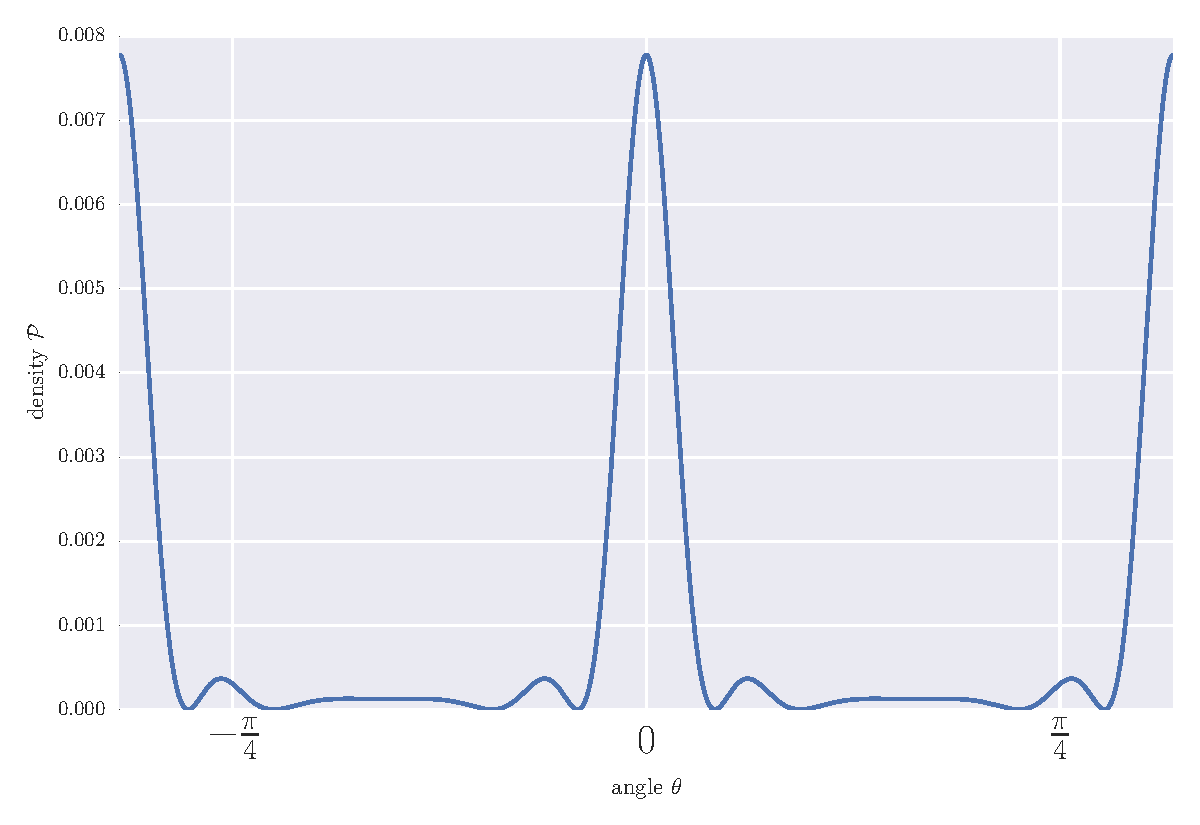
\includegraphics[width=0.8\linewidth]{figures/sinc1}
    \caption{This is the theoretic intensity distribution following equation~\eqref{eq:sinc1}. 
        We plugged in $\lambda = 632.8$nm and $b = 1 \mu$m. The density is normed to one.}
    \label{fig:sinc1}
\end{figure}
\paragraph{diffraction gratings} 
Equation~\eqref{eq:sinc1} leads straigtfoward to the intensity density of
the diffraction grating, using \eqref{eq:fourier}. We need to understand 
that a diffraction grating is the result of convoluting of a simple opening
(using the $\Theta$ function which is one for $x>0$ and zero otherwise)
\begin{align}
    \label{eq:multisplit}
    g_b(x) &= \Theta(x - \frac{b}{2}) - \Theta( \frac{b}{2} - x ) \qquad
           &\text{Single split} \\ 
   g(x)   &:= \sum_{n=0}^{N-1} g_b(x-nK) 
         \qquad &\text{Multi split with spacing } K
\end{align}
Calculating straightforward we would have:
\begin{equation}
    \psi(\theta) = \sum_{n = 0}^{N-1}  \int^{n \cdot K + b}_{0} e^{i k x sin(\theta)} \del x
\end{equation}
which simplifies (after some none trivial steps):
\begin{equation}
    I(\theta) \propto \psi(\theta)^2 \propto \sinc(\beta)^2 \left (\frac{\sin(N\gamma)}{N \sin(\gamma)}\right )^2
\end{equation}
with
\begin{equation}
    \beta = \frac{k}{2}b \sin(\theta) \quad \text{and} \quad \gamma = k\cdot K \sin(\theta).
\end{equation}
Since $K \sin (\theta)$ is the length of the light to the respecting point on the screen, every time
this distance is equal to an multiple of the wavelength, we will have a maximum:
\begin{equation}
    m \lambda = K \sin(\theta) \quad \text{ with }m \in \mathbb{Z}
    \label{eq:N_lines_interference}
\end{equation}
\clearpage
\subsection{Acoustooptics}
\begin{SCfigure}
    \centering
    \caption{Illustration of the acousto-optic effect: The former transparent and homogenious medium is
        excited by an acoustic wave (turquoise) which changes the dielectric constant. On the top you notice
        the blue line which indicates an incident ligthbeam by an angle $\theta$. Obviously this change
        of the refractive index is due to the dieletric constant is connected to diffractive phenomena like
        gratings, but in a non-trivial way. The main point here is that the angle $\theta$ should be low enough
        for the ligthbeam not to be scattered (this would lead to bragg-like scattering) which is at the moment
        not interesting for us. }
    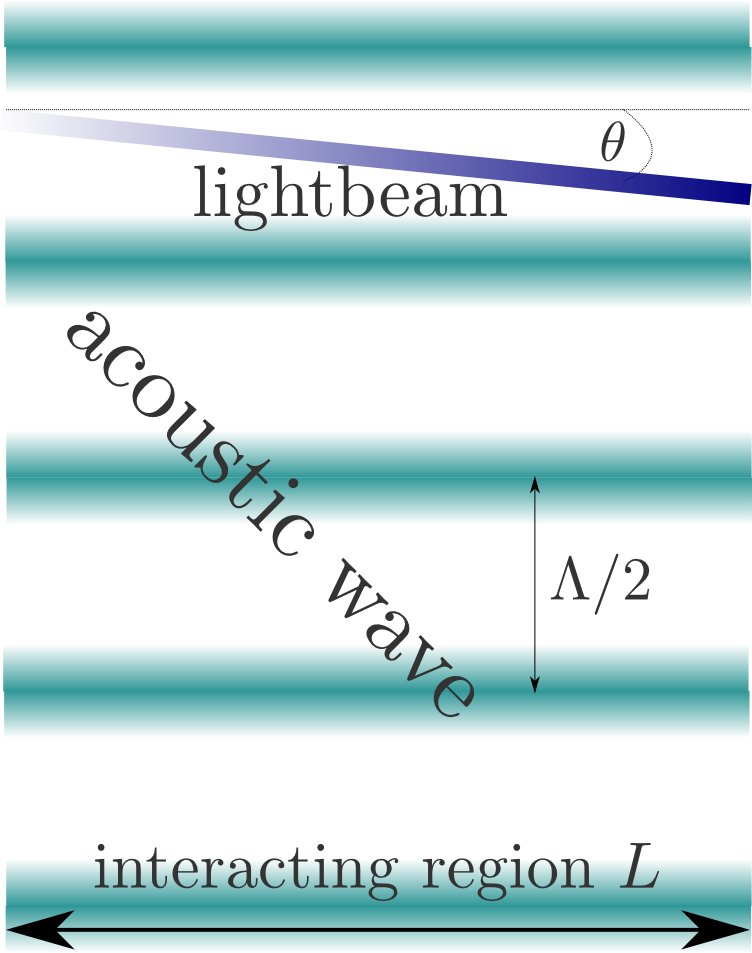
\includegraphics[width=0.5\linewidth]{figures/ramannath1.png}
    \label{fig:ramannath1}
\end{SCfigure}
Considering a density variation in a material due to an acoustic wave, the dieletric constant is will
change respectively (following \cite{boyd2003nonlinear} closely). 
Incidident optical waves are diffracted or scattered, depending on the spatial curvature
of the dielectric constant (see figure~\ref{fig:ramannath1}). The condition for scattering not to occure can
be estimated: Using the acoustic wavelength $\Lambda$ and the optic wavelength $\lambda$ we introduce 
\begin{equation}
    \label{eq:deltatheta}
    \delta \theta = \frac{\lambda}{\Lambda}
\end{equation}
as the characteristic angular spread of the diffracted light. Scattering cannot occur, when 
\begin{equation}
    \delta \theta L < \Lambda.
\end{equation}
Which we can plugin into \eqref{eq:deltatheta} to get
\begin{equation}
    \frac{\lambda L}{\Lambda^2} < 1
\end{equation}
Now we chose the density fluctuations to be 
\begin{equation}
    \Delta \tilde{n}(z,t) = 2 \Delta n \sin(q z - \Omega t)
\end{equation}
where we introduced the tilde refers to the time dependency, while $\Delta n$ denotes the timeindepend part.
$\Omega$ refers to the frequency and $q$ to the spatial wave vector of the acoustic wave.
The incident light can now be represented by (solution of onbounded laplace)
\begin{equation}
    \tilde{E}(r,t) = A e ^{i(kx - \omega t)} + A^{*}e ^{-i(kx - \omega t)}.
\end{equation}
Obviously passing through the interacting region $L$ the optical wave picks up a phase 
\begin{equation}
    \phi = \Delta \tilde{n}\frac{\omega}{c}L = \Delta n \frac{\omega}{c}L \sin (qz - \Omega t).
\end{equation}
The final and critical step is to use the \textbf{Jacobi-Anger expansion}
\begin{equation}
    e^{i\delta \sin y} = \sum_{l = -\infty}^{\infty} J_l(\delta)e^{ily} 
\end{equation}
where we used the Bessel function of first kind
\begin{equation}
J_\alpha(x) = \sum_{m=0}^\infty \frac{(-1)^m}{m! \, \Gamma(m+\alpha+1)} {\left(\frac{x}{2}\right)}^{2m+\alpha}.
\end{equation}
Plugging in the last two equations we can look at the electromagnetic wave after surpassing: 
\begin{equation}
    \tilde{E}(r,t)=A \sum_{l = -\infty}^{\infty} J_l(\delta)e^{i
        \left [kx -\omega t + \delta \sin(qz - \Omega t) \right ]  } + \quad \text{complex conjugates}
\end{equation}
where we have defined
\begin{equation}
    \delta = 2\Delta n \omega L / c.
\end{equation}
The maxima of this pattern are analogous to the diffraction grating:
\begin{equation}
    \sin(\theta) = \frac{\lambda}{\Lambda} m \qquad m \in \mathbb{Z}
\end{equation}
And the intensity peaks are given by
\begin{equation}
    I_l = |A|^2 J_l(\delta)^2
\end{equation}
